% Options for packages loaded elsewhere
\PassOptionsToPackage{unicode}{hyperref}
\PassOptionsToPackage{hyphens}{url}
\PassOptionsToPackage{dvipsnames,svgnames,x11names}{xcolor}
%
\documentclass[
]{article}
\title{Predicting readmission probability for diabetes inpatients}
\author{Annie Vo \and Sarah Hayward \and Jessica Brown}
\date{}

\usepackage{amsmath,amssymb}
\usepackage{lmodern}
\usepackage{iftex}
\ifPDFTeX
  \usepackage[T1]{fontenc}
  \usepackage[utf8]{inputenc}
  \usepackage{textcomp} % provide euro and other symbols
\else % if luatex or xetex
  \usepackage{unicode-math}
  \defaultfontfeatures{Scale=MatchLowercase}
  \defaultfontfeatures[\rmfamily]{Ligatures=TeX,Scale=1}
\fi
% Use upquote if available, for straight quotes in verbatim environments
\IfFileExists{upquote.sty}{\usepackage{upquote}}{}
\IfFileExists{microtype.sty}{% use microtype if available
  \usepackage[]{microtype}
  \UseMicrotypeSet[protrusion]{basicmath} % disable protrusion for tt fonts
}{}
\makeatletter
\@ifundefined{KOMAClassName}{% if non-KOMA class
  \IfFileExists{parskip.sty}{%
    \usepackage{parskip}
  }{% else
    \setlength{\parindent}{0pt}
    \setlength{\parskip}{6pt plus 2pt minus 1pt}}
}{% if KOMA class
  \KOMAoptions{parskip=half}}
\makeatother
\usepackage{xcolor}
\IfFileExists{xurl.sty}{\usepackage{xurl}}{} % add URL line breaks if available
\IfFileExists{bookmark.sty}{\usepackage{bookmark}}{\usepackage{hyperref}}
\hypersetup{
  pdftitle={Predicting readmission probability for diabetes inpatients},
  pdfauthor={Annie Vo; Sarah Hayward; Jessica Brown},
  colorlinks=true,
  linkcolor={Maroon},
  filecolor={Maroon},
  citecolor={Blue},
  urlcolor={blue},
  pdfcreator={LaTeX via pandoc}}
\urlstyle{same} % disable monospaced font for URLs
\usepackage[margin=1in]{geometry}
\usepackage{graphicx}
\makeatletter
\def\maxwidth{\ifdim\Gin@nat@width>\linewidth\linewidth\else\Gin@nat@width\fi}
\def\maxheight{\ifdim\Gin@nat@height>\textheight\textheight\else\Gin@nat@height\fi}
\makeatother
% Scale images if necessary, so that they will not overflow the page
% margins by default, and it is still possible to overwrite the defaults
% using explicit options in \includegraphics[width, height, ...]{}
\setkeys{Gin}{width=\maxwidth,height=\maxheight,keepaspectratio}
% Set default figure placement to htbp
\makeatletter
\def\fps@figure{htbp}
\makeatother
\setlength{\emergencystretch}{3em} % prevent overfull lines
\providecommand{\tightlist}{%
  \setlength{\itemsep}{0pt}\setlength{\parskip}{0pt}}
\setcounter{secnumdepth}{-\maxdimen} % remove section numbering
\ifLuaTeX
  \usepackage{selnolig}  % disable illegal ligatures
\fi

\begin{document}
\maketitle

{
\hypersetup{linkcolor=}
\setcounter{tocdepth}{4}
\tableofcontents
}
\begin{itemize}
\tightlist
\item
  to hide source code: echo = FALSE
\item
  to hide text output: results = `hide' or results = FALSE
\item
  hide messages: message = FALSE
\item
  hide warning messages: warning = FALSE
\item
  hide plotsL fig.show = `hide'
\end{itemize}

\hypertarget{executive-summary}{%
\section{Executive Summary}\label{executive-summary}}

\hypertarget{data-summary-eda}{%
\section{Data Summary / EDA}\label{data-summary-eda}}

\begin{itemize}
\tightlist
\item
  Nature of the data, origin
\item
  Necessary quantitative and graphical summaries
\item
  Are there any problems with the data?
\item
  Which variables are considered as input
\end{itemize}

Let's look at what other variables should be factors

Here we note that 2273 patients have an unidentified race

The original data is from the
\href{https://archive.ics.uci.edu/ml/datasets/Diabetes+130-US+hospitals+for+years+1999-2008}{Center
for Clinical and Translational Research} at Virginia Commonwealth
University. It covers data on diabetes patients across 130 U.S.
hospitals from 1999 to 2008. There are over 100,000 unique hospital
admissions in this dataset, from \textasciitilde70,000 unique patients.
The data includes demographic elements, such as age, gender, and race,
as well as clinical attributes such as tests conducted,
emergency/inpatient visits, etc.

For our analysis we will use a cleaned subset of this dataset which
excludes variables with lots of missing values and variables with very
little variability, as well as applying binning on some categorical
variables.

The event of interest is \textbf{readmitted within \textless{} 30 days}.

\includegraphics{Diabetes-Project-Code_files/figure-latex/unnamed-chunk-6-1.pdf}

\includegraphics{Diabetes-Project-Code_files/figure-latex/unnamed-chunk-7-1.pdf}

\includegraphics{Diabetes-Project-Code_files/figure-latex/unnamed-chunk-8-1.pdf}

\includegraphics{Diabetes-Project-Code_files/figure-latex/unnamed-chunk-9-1.pdf}

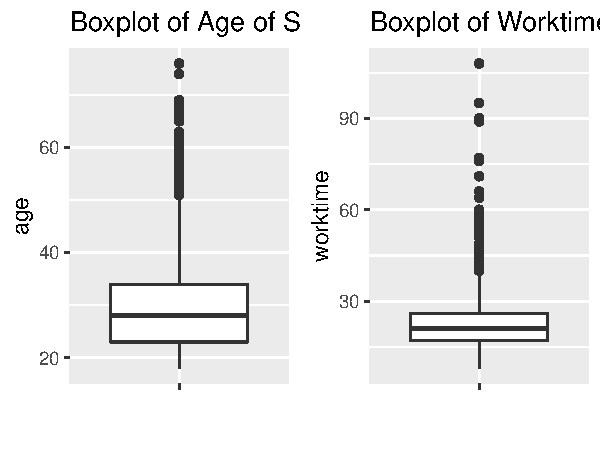
\includegraphics{Diabetes-Project-Code_files/figure-latex/unnamed-chunk-10-1.pdf}

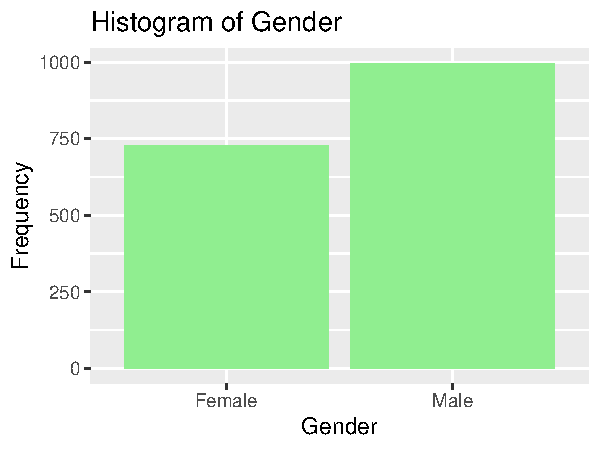
\includegraphics{Diabetes-Project-Code_files/figure-latex/unnamed-chunk-11-1.pdf}
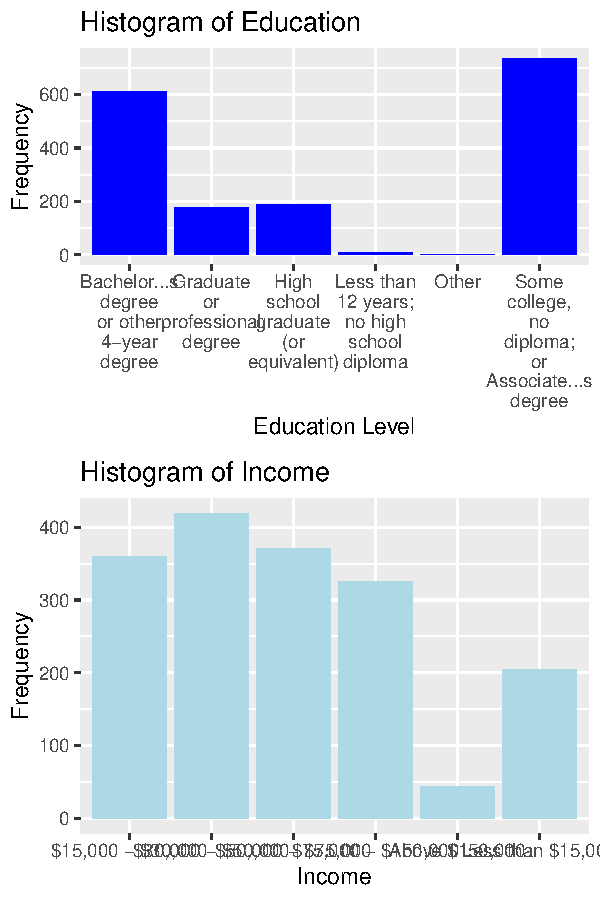
\includegraphics{Diabetes-Project-Code_files/figure-latex/unnamed-chunk-12-1.pdf}

\hypertarget{analysis}{%
\section{Analysis}\label{analysis}}

\begin{itemize}
\tightlist
\item
  Various appropriate statistical methods: e.g.~glmnet
\item
  Comparisons various models
\item
  Final model(s)
\end{itemize}

\hypertarget{conclusion}{%
\section{Conclusion}\label{conclusion}}

\begin{itemize}
\tightlist
\item
  Summarize results and the final model
\item
  Final recommendations
\end{itemize}

\hypertarget{appendix}{%
\section{Appendix}\label{appendix}}

\begin{itemize}
\tightlist
\item
  Any thing necessary to keep but for which you don't want them to be in
  the main report
\item
  Use Appendices to display lengthy output.
\end{itemize}

\end{document}
